\documentclass{beamer}
\usepackage[english]{babel}
\usepackage[utf8]{inputenc}
\usepackage[T1]{fontenc}
\usepackage{lmodern}
\usepackage{url}
\usepackage{graphicx}

\usepackage{amsmath}
\usepackage{amsthm}
\usepackage{amsfonts}
\usepackage{subfigure}

\newcommand{\R}{\mathbb R}
\newcommand{\N}{\mathbb N}
\newcommand{\Z}{\mathbb Z}
\newcommand{\C}{\mathbb C}
\newcommand{\Q}{\mathbb Q}
\newcommand{\f}{\mathcal F}
%\newcommand{\P}{\mathbb P}

\mode<presentation>
{
    \usetheme{CambridgeUS}
    \usecolortheme{seahorse}
}

\title[VaR on option portfolio]
{VaR on option portfolio}

\author[Tia Krofel, Brina Ribič, Matej Rojec]
{\textbf{Authors: Tia Krofel, Brina Ribič, Matej Rojec} \\
\textbf{Mentor: dr. Aleš Ahčan}
}


\institute[] 
{
  University of Ljubljana\\
  School of Economics and Business\\
  Slovenia
}

\date[20. december 2022]

\begin{document}

\begin{frame}
  \titlepage
\end{frame}

\section{Framework}

\begin{frame}
    \frametitle{Options}
    \begin{block}<1->{Option}
        An option gives its owner the right, but not the obligation, to call (buy)
        or put (sell) an underlying asset at a strike price on a fixed expiration date. 
    \end{block}
    \begin{itemize}
        \item<3-> european options
        \item<4-> american options
        \item<5-> exotic options
    \end{itemize}
\end{frame}

\begin{frame}
    \frametitle{European options}
    Value of european option at its expiration time:
    \begin{itemize}
        \item<1-> Call: $C_T = \max\{S_T-K,0\}$
        \item<2-> Put: $P_T = \max\{K-S_T,0\}$
    \end{itemize}
\end{frame}

\begin{frame}
    \frametitle{Black-Scholes model}
    Price of european call option:
    \begin{itemize}
        \item $V_t = S_t\Phi(d_1) - Ke^{-R(T-t)}\Phi(d_2)$
        \begin{itemize}
            \item $K$ \dots strike price
            \item $R$ \dots risk-free interest rate
            \item $S_t$ \dots the underlying asset's value at time $t$
        \end{itemize}
        \item $d_1 = \frac{\ln(\frac{S_0}{K}e^{RT})+\frac{\sigma^2}{2}T}{\sigma\sqrt{T}}$
        \item $d_2 = d_1-\sigma\sqrt{T}$
    \end{itemize}
\end{frame}

\begin{frame}
    \frametitle{VaR}
    \begin{block}{VaR definiton}
        Let $X$ be a random variable on a probability space $(\Omega, \f, \mathcal{P})$ and $\alpha \in (0, 1)$.
        $\text{VaR}_\alpha(X)$ is defined as the $(1-\alpha)$ quantile of -$X$. Then
        $$
        \text{VaR}_\alpha(X) := - \inf \{ x \in \R \mid F_X(x) > \alpha \} = F^{-1}_{-X}(1-\alpha).
        $$
    \end{block}
\end{frame}

\begin{frame}
    \frametitle{Non-linear VaR}
    \begin{figure}\label{payoff}
        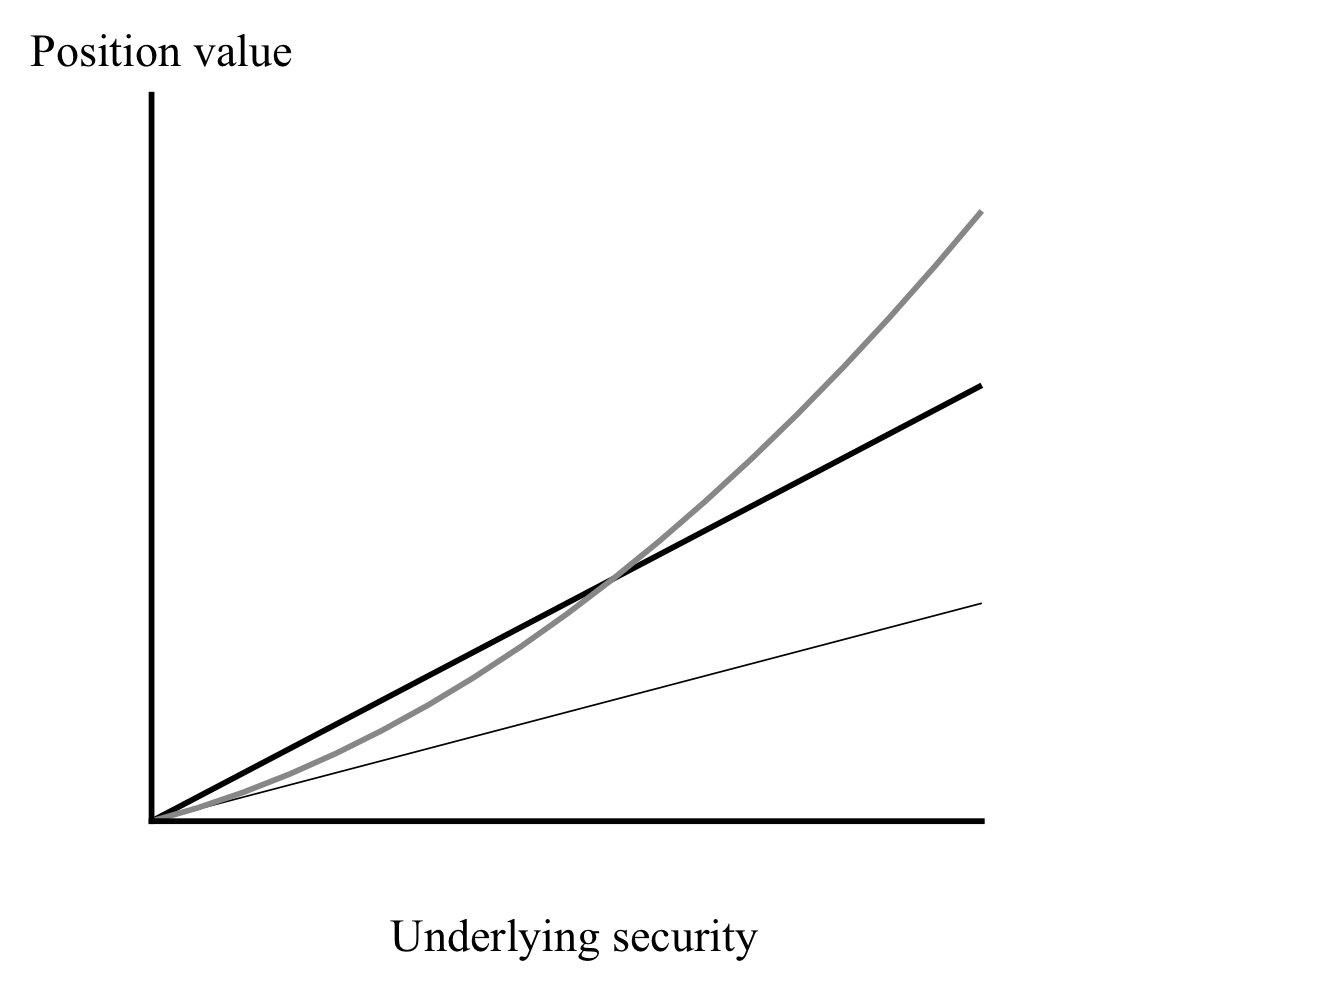
\includegraphics[width=0.7\textwidth]{payoff.jpg}
        \caption{Linear and non-linear function of payoff.}
    \end{figure}
\end{frame}

\section{The Greeks}

\begin{frame}
    \frametitle{The Delta}
    The Delta of an option tells us how much an option price 
    would change relative to a change in the price of the 
    underlying asset.\pause
    

    \begin{block}{}
        $$
        \Delta = \frac{\partial V}{\partial S}
        $$ 
    \end{block}
    \begin{itemize}
        \item<3-> Call: $\Delta\in [0,1]$
        \item<4-> Put: $\Delta\in [-1,0]$
        \item<5-> European call option: $\Phi(d_1)$
    \end{itemize}
\end{frame}

\begin{frame}
    \frametitle{The Gamma}
    The Gamma measures the change in an option's 
    delta relative to changes in the underlying
    asset price.\pause

    \begin{block}{}
        $$
        \Gamma = \frac{\partial^2 V}{\partial S^2}
        $$
    \end{block}
    \pause
    \begin{itemize}
        \item European call option: $e^{-R(T-t)}\frac{\Phi(d1)}{S_t\sigma\sqrt{T-t}}$
    \end{itemize}
    \vspace{0.3cm}
    \pause 
    In general, the gamma is at its maximum point when the stock is near the 
    strike of the option.
\end{frame}

\begin{frame}
    \frametitle{The Theta}
    The Theta measures an options sensitivity to time 
    and tells us how susceptible is an option's value 
    to the passage of time.\pause

    \begin{block}{}
        $$
        \Theta = \frac{\partial V}{\partial t}
        $$  
    \end{block}\pause
    \vspace{0.3cm}
    \begin{itemize}
        \item An option's potential drops as time moves on. 
    \end{itemize}\pause
    \vspace{0.3cm}
    Long positions generally have a negative theta and 
    short positions a positive one.
    
\end{frame}

\begin{frame}
    \frametitle{The Vega}
    The Vega measures an options sensitivity to volatility.\pause

    \begin{block}{}
        $$ 
        \mathcal{V}  = \frac{\partial V}{\partial \sigma}
        $$  
    \end{block}\pause
    \vspace{0.3cm}
    As an amount by which the option price changes when the 
    volatility changes, vega is always a positive number.
\end{frame}

\begin{frame}
    \frametitle{Delta-Gamma-Theta Approach}
    Incorporation of greek parameters into the VaR can 
    provide a more accurate estimaet of the risk of loss 
    on option portfolio.

    \vspace{0.3cm}
    \pause
    Importance of the three Greeks used for VaR calculation:
    \vspace{0.3cm}
    \pause
    \begin{itemize}
        \item Delta: the potential change 
        in the option's value associated with a 
        unit shift in the underlying asset's price;\pause
        \item Gamma: important role in 
        VaR calculations as the underlying asset price 
        fluctuates more significantly;\pause
        \item Theta: time decay is a major factor
        in the approximation of the overall risk of the portfolio.
    \end{itemize}
\end{frame}

\end{document}